\section{TDM MIMO FMCW Theory}
\label{sec:rationale}

This section provides the signal-processing foundations that underpin our differentiable renderer, included for readers whose background is primarily in rendering or vision rather than radar.
Sec.~\ref{sec:supp_fmcw} derives the FMCW beat signal that the renderer must synthesize per traced path.
Sec.~\ref{sec:supp_iq} explains IQ demodulation, which determines why the renderer outputs \emph{complex}-valued ADC samples.
Sec.~\ref{sec:tdm_mimo_imaging} shows how these ADC samples are transformed into the 2D range--azimuth and 3D range--azimuth--elevation images used in our training loss (Eq.~\ref{eq:ra_loss}) and evaluation metrics.
Sec.~\ref{sec:supp_mc_derivation}--\ref{sec:supp_power_to_adc} derive the Monte Carlo estimator (main paper Eq.~3) and the power-to-ADC conversion that closes the forward model.
Readers familiar with FMCW radar may skip directly to Sec.~\ref{sec:supp_implementation}.

\subsection{FMCW Formulation}
\label{sec:supp_fmcw}

We summarize the standard FMCW signal model following~\cite{skolnik2001introduction,dudek2010millimeter}. FMCW radars emit a linearly frequency-modulated chirp into the scene,
\begin{equation}
    s(t) = A_s \cos\!\left(2\pi f_c t + \pi K t^2 \right), 
\end{equation}
for $\qquad 0 < t < T_c,$ and receive a delayed echo
\begin{equation}
    u(t) = A_r \cos\!\left(2\pi f_c (t-\tau) + \pi K (t-\tau)^2 \right), 
\end{equation}
for $\qquad \tau < t < T_c$, where $K$ is the chirp slope, $f_c$ is the start frequency, $T_c$ is the chirp duration, and $\tau = 2 d(t)/c$ is the round-trip delay for a target at range $d$ and wave propagation speed $c$. The total swept bandwidth is
\begin{equation}
    B = f_{\max} - f_{\min} = (f_c + K T_c) - f_c = K T_c.
\end{equation}

When the received chirp is mixed with the (still transmitting) chirp and low-pass filtered, the resulting real-valued beat signal is
\begin{equation}
    m_{\mathrm{R}}(t) \approx A_m 
    \cos\!\left(2\pi K \tau\, t + 2\pi f_c \tau - \pi K \tau^2\right),
    \label{eq:real_beat}
\end{equation}
for $\qquad \tau < t < T_c,$ where $A_m$ subsumes constant amplitude factors. The beat frequency is
\begin{equation}
    f_{\mathrm{IF}} = K \tau = \frac{2 K d}{c},
\end{equation}
and the range-dependent phase is dominated by
\begin{equation}
    \phi(t) \approx 2\pi f_c \tau = 4\pi \frac{d}{\lambda},
\end{equation}
with carrier wavelength $\lambda = c/f_c$. The small quadratic term $\pi K \tau^2$ is typically negligible for automotive-range targets ($K\tau^2 \ll f_c\tau$).

\begin{figure}[t]
  \centering
  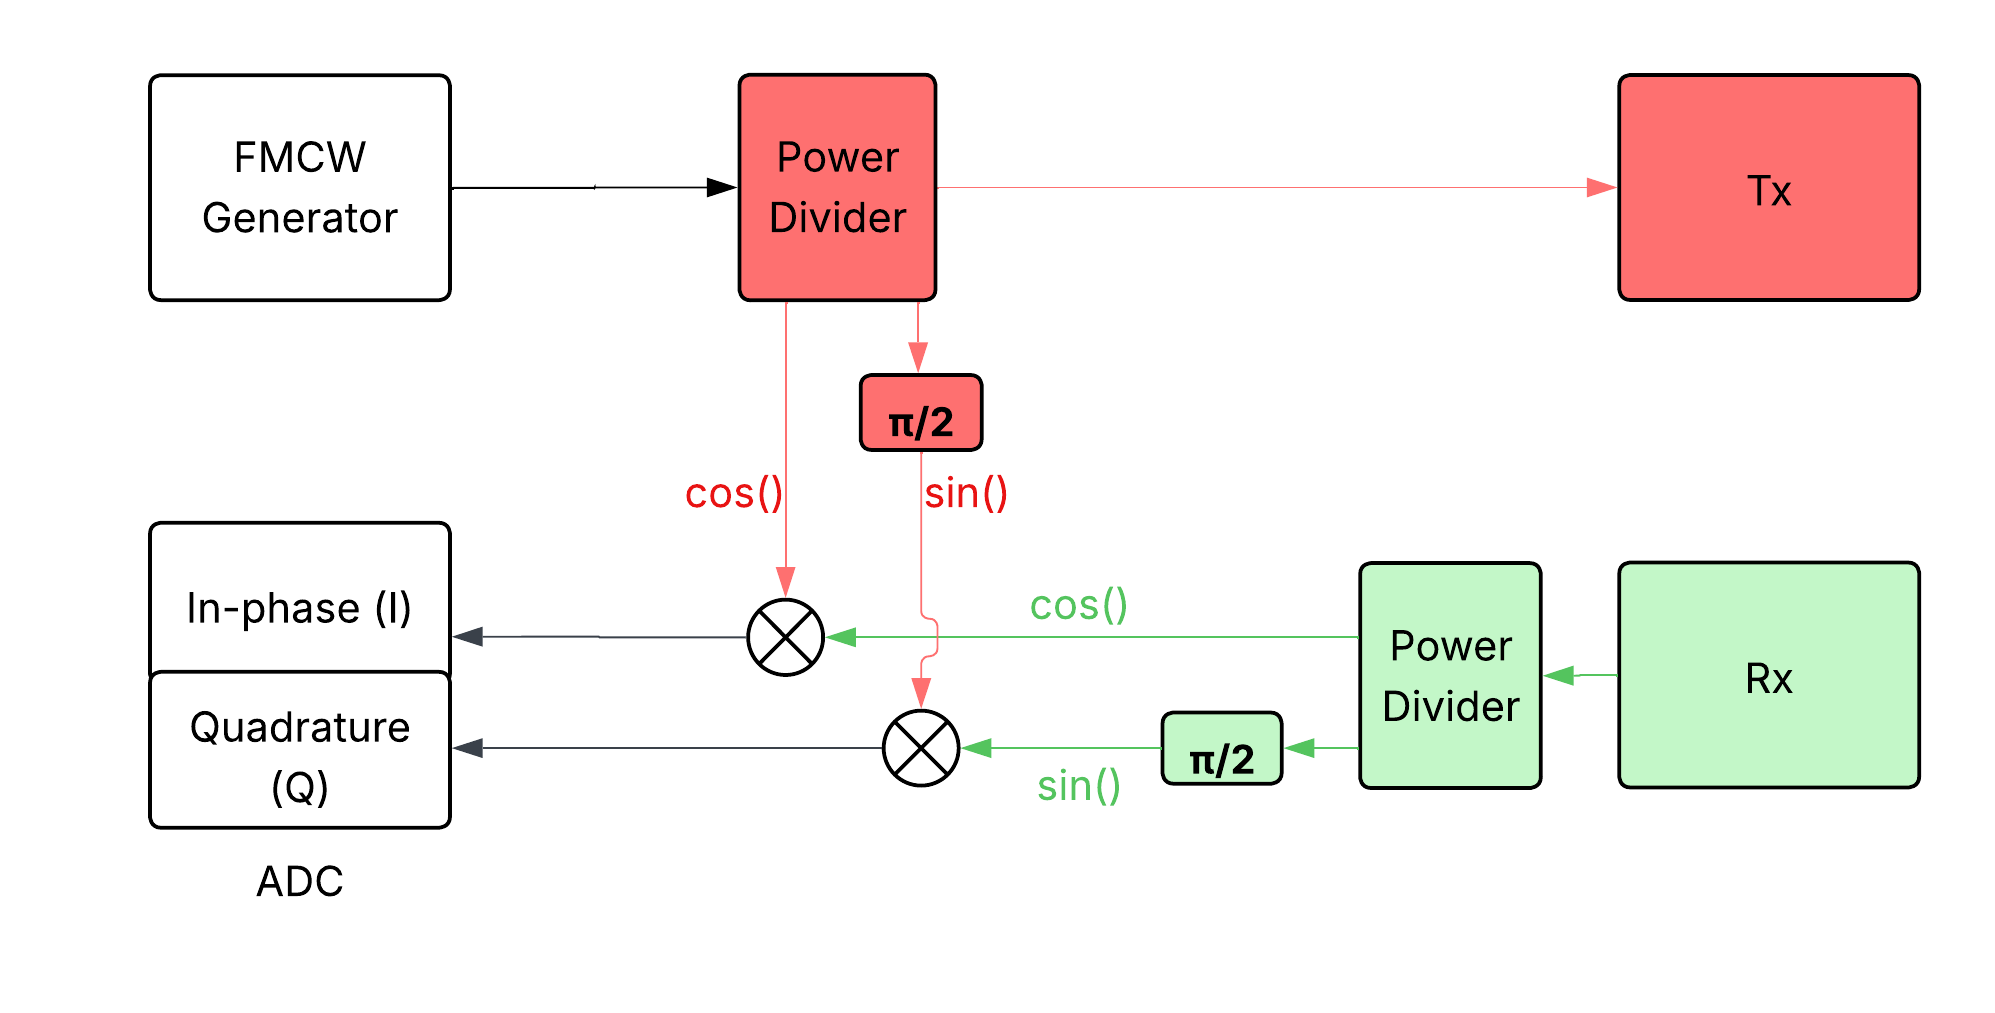
\includegraphics[width=\linewidth]{figs/IQ_demodulation.png}
  \caption{Block diagram of IQ demodulation in FMCW radar. The received echo is mixed with in-phase (I) and quadrature (Q) copies of the transmit chirp and low-pass filtered, producing complex baseband samples that preserve both amplitude and phase for downstream range and angle processing.}
  \label{fig:iq_demod}
\end{figure}

\subsection{IQ Demodulation for Complex Baseband ADC}
\label{sec:supp_iq}

In practice, the RF front-end uses IQ demodulation as shown in Fig.~\ref{fig:iq_demod}. A single real mixer would fold the symmetric RF sidebands at $\pm f_{\mathrm{IF}}$ onto the same baseband frequencies, effectively aliasing positive and negative beat frequencies onto the same baseband bins. IQ mixing instead produces a complex-valued baseband signal with a one-sided spectrum, keeping positive and negative frequencies separated, improving SNR, and yielding an unambiguous mapping between beat frequency and range~\cite{270463, alizadeh2019remote}.

A copy of the transmit chirp is routed to the local-oscillator (LO) ports of two mixers: one LO branch uses a cosine (in-phase, I) and the other a $90^\circ$-shifted sine (quadrature, Q). The received RF signal is applied to the RF port of both mixers, and each output is low-pass filtered and digitized, yielding
\begin{align}
    I(t) &\propto \cos\!\big(2\pi f_{\mathrm{IF}} t + \phi(t)\big),\\
    Q(t) &\propto \sin\!\big(2\pi f_{\mathrm{IF}} t + \phi(t)\big).
\end{align}
Interpreting these as the real and imaginary parts of a single complex baseband beat signal,
\begin{equation}
    m(t) = I(t) + j\,Q(t),
\end{equation}
is equivalent to multiplying the received RF with a complex LO and discarding the image band.

To make this analytic form explicit, we write the transmitted and received chirps using Euler’s formula following~\cite{270463}:
\begin{align}
    s(t) &= A_s \exp\!\big(j (2\pi f_c t + \pi K t^2)\big),\\
    u(t) &= A_r \exp\!\big(j [2\pi f_c (t-\tau) + \pi K (t-\tau)^2]\big).
\end{align}
Ideal IQ demodulation corresponds to mixing the received signal with the complex conjugate of the transmit signal:
\begin{equation}
    m(t) = u(t)\,s^*(t).
\end{equation}
Using the phase difference between $u(t)$ and $s(t)$, this simplifies to
\begin{align}
    m(t) 
    &= A_s A_r \exp\!\left(
        j \left[ 2\pi K \tau\, t + 2\pi f_c \tau - \pi K \tau^2 \right]
    \right) \\
    &\approx A_m \exp\!\left(
        j \left[ 2\pi f_{\mathrm{IF}} t + \phi(t) \right]
    \right),
    \label{eq:complex_baseband_continuous}
\end{align}
where again $f_{\mathrm{IF}} = K \tau = 2 K d/c$ and $\phi(t) \approx 4\pi d/\lambda$.

Finally, the ADC samples this complex baseband signal at rate $f_s$, producing discrete-time IQ data
\begin{equation}
    m[n] \approx A_m 
    \exp\!\left(
        j \left[ 2\pi f_{\mathrm{IF}} \frac{n}{f_s} + \phi[n] \right]
    \right),
    \label{eq:adc_samples}
\end{equation}
where $n$ indexes fast-time samples within a chirp and $\phi[n]$ encodes the path-length-dependent phase (and any slow motion) at the $n$-th sample. These complex ADC samples are the starting point for our subsequent MIMO imaging formulation.


\subsection{TDM MIMO for 2D and 3D Imaging}
\label{sec:tdm_mimo_imaging}

The complex ADC samples in~\eqref{eq:adc_samples} describe a single transmit--receive pair observing a single target. Modern mmWave sensors instead use multiple transmit (TX) and receive (RX) antennas arranged in an array and operate them in time-division multiplexing (TDM) mode to synthesize a larger \emph{virtual} aperture. This enables 2D and 3D spatial imaging via discrete Fourier transforms over carefully chosen dimensions of the ADC data cube, as described by~\cite{9658500}.

\paragraph{TDM MIMO data cube.}
Let $N_\text{TX}$ and $N_\text{RX}$ denote the number of physical transmitters and receivers, $N_\text{chirp}$ the number of chirps in a frame, and $N_\text{s}$ the number of fast-time ADC samples per chirp. In a TDM sequence, only one TX is active at a time. Each chirp slot is assigned to a particular transmitter, cycling through all $N_\text{TX}$ elements.

For TX element $i \in \{0,\dots,N_\text{TX}-1\}$, RX element $j \in \{0,\dots,N_\text{RX}-1\}$, chirp index $\ell \in \{0,\dots,N_\text{chirp}-1\}$, and fast-time sample index $n \in \{0,\dots,N_\text{s}-1\}$, the sampled complex beat signal can be written as
\begin{equation}
    m_{ij}[\ell,n] \approx A_{ij}[\ell]\,
    \exp\!\left(
        j\left[
            2\pi f_{\mathrm{IF}} \frac{n}{f_s}
            + \phi_{ij}[\ell]
        \right]
    \right),
    \label{eq:tdm_mimo_sample}
\end{equation}
where $f_s$~is the ADC sampling rate, $A_{ij}[\ell]$~captures path loss and BSDF/antenna gains, and the phase~$\phi_{ij}[\ell]$ contains the range phase~$4\pi d/c$ plus offsets from TX/RX array geometry and slow motion across chirps.

Stacking all $(i,j,\ell,n)$ produces a four-dimensional data block. For convenience, the TX/RX indices are often flattened into a \emph{virtual} antenna index $v \in \{0,\dots,N_\text{V}-1\}$ with $N_\text{V} = N_\text{TX} N_\text{RX}$, giving $m_v[\ell,n]$.

\paragraph{Range FFT (fast-time).}
The first processing step is a 1D FFT along fast time $n$ for each virtual channel $v$ and chirp $\ell$, which converts beat frequency to range. Before the FFT, a Hann window $w_\text{R}[n]$ is applied in fast time to suppress spectral leakage and sidelobes:
\begin{equation}
    M_v[\ell,k]
    =
    \sum_{n=0}^{N_\text{s}-1}
        w_\text{R}[n]\,
        m_v[\ell,n]\,
        \exp\!\left(
            -j \frac{2\pi}{N_\text{s}} k n
        \right),
    \label{eq:range_fft}
\end{equation}
$\qquad k = 0,\dots,N_\text{s}-1.$ Each frequency bin $k$ corresponds to a range
\begin{equation}
    R_k = \frac{c\,k}{2B},
    \label{eq:range_bin}
\end{equation}
so the magnitude $\lvert M_v[\ell,k]\rvert$ encodes the reflectivity at range $R_k$ observed by virtual channel $v$. Range estimation is therefore driven primarily by the \emph{amplitude} of the fast-time FFT, while the complex phase of $M_v[\ell,k]$ is carried forward for angle processing.

\paragraph{Angle-of-arrival from virtual array phase.}
At a fixed range bin $k$, a far-field target arriving from direction $(\theta,\varphi)$ (azimuth and elevation) produces nearly identical amplitudes across the virtual aperture but a systematic phase ramp tied to the projection of the direction vector onto each element’s position. For a 1D linear virtual array along $x$ with inter-element spacing $d_x$, the phase at element $v$ satisfies
\begin{equation}
    \phi_v(k) \approx \phi_0(k) 
    + \frac{2\pi}{\lambda}\, x_v \sin\theta,
\end{equation}
where $x_v$ is the $x$-coordinate of virtual element $v$. Taking a DFT over the virtual array index therefore steers beams in angle:
\begin{align}
\widetilde{M}[k,n_\theta]
&=
\sum_{v=0}^{N_\mathrm{V}-1}
    w_\mathrm{AZ}[v]\,
    \Big(
        \frac{1}{N_\text{chirp}}
        \sum_{\ell=0}^{N_\text{chirp}-1}
            M_v[\ell,k]
    \Big)
    \nonumber\\
&\quad\times
    \exp\!\left(
        -j \frac{2\pi}{N_\mathrm{V}} n_\theta v
    \right),
\label{eq:azimuth_fft}
\end{align}

where $w_\text{AZ}[v]$ is a spatial (e.g., Hann) window applied across the virtual aperture to reduce angular sidelobes. The bin index $n_\theta$ maps to azimuth angle via the usual array steering relation,
\begin{equation}
    \theta_{n_\theta}
    \approx \sin^{-1}\!\left(
        \frac{\lambda}{N_\text{V} d_x}\, n_\theta
    \right),
\end{equation}
assuming half-wavelength spacing and small-angle approximation. Here, the \emph{relative phase} of $M_v[\ell,k]$ across $v$ is what encodes direction-of-arrival. The FFT over $v$ converts this phase gradient into an angular spectrum. The result $\lvert \widetilde{M}[k,n_\theta]\rvert$ is a 2D range--azimuth (RA) map.

When the physical TX and RX antennas are arranged in a 2D grid, TDM MIMO produces a 2D virtual array indexed by $(v_x,v_z)$ along horizontal and vertical baselines with spacings $d_x$ and $d_z$. After the range FFT, two consecutive spatial FFTs over $v_x$ and $v_z$ yield a 3D range--azimuth--elevation (RAE) cube:
\begin{align}
\widetilde{M}_x[k,n_\theta,v_z]
&=
\sum_{v_x} w_\text{AZ}[v_x]\,
    \bar{M}[k,v_x,v_z]\,
    \nonumber\\
&\quad\times
    \exp\!\left(
        -j \frac{2\pi}{N_x} n_\theta v_x
    \right),
\label{eq:mx_fft}
\\[0.3em]
\widetilde{M}_{xz}[k,n_\theta,n_\phi]
&=
\sum_{v_z} w_\text{EL}[v_z]\,
    \widetilde{M}_x[k,n_\theta,v_z]\,
    \nonumber\\
&\quad\times
    \exp\!\left(
        -j \frac{2\pi}{N_z} n_\phi v_z
    \right).
\label{eq:mxz_fft}
\end{align}

with $N_x$ and $N_z$ the number of virtual elements in azimuth and elevation, and $w_\text{EL}[v_z]$ an elevation window. The indices $(n_\theta,n_\phi)$ map to azimuth and elevation angles via the corresponding steering relations. In our pipeline, these RA/RAE tensors are obtained by applying Hann windows in each FFT dimension to suppress sidelobes and then using the magnitudes $\lvert \widetilde{M} \rvert$ for downstream 2D/3D imaging.

\paragraph{Slow-time (Doppler) dimension.}
For moving targets, the chirp index $\ell$ carries an additional phase term proportional to radial velocity. A further FFT along $\ell$ recovers Doppler frequency and yields range-Doppler-angle cubes commonly used in automotive tracking. In this work, we do not model the motion of the radar via an additional Doppler phase term, nor do we apply a Doppler FFT over all chirps. Instead, our inverse renderer assumes static scenes even though the data was collected from a moving platform, and we therefore partially attribute residual differences between rendered and ground-truth ADC to this simplification. For 2D/3D spatial imaging, we apply only the fast-time FFT for range and the virtual-array FFTs for azimuth and elevation, all acting on the same complex baseband ADC samples in~\eqref{eq:tdm_mimo_sample}.

\subsection{Bistatic Radar Equation: From RCS to MC Estimator}
\label{sec:supp_mc_derivation}

This section provides the full derivation of the Monte Carlo estimator used in the main paper (Eq.~3). We follow an RX-centric formulation where rays are traced from the receiver.

\paragraph{Area-domain form.}
For a single TX--RX pair observing a surface point $\mathbf{x}$ with normal $\mathbf{n}$, distances $d_t = \|\mathbf{x} - \mathbf{x}_{tx}\|$ and $d_r = \|\mathbf{x}_{rx} - \mathbf{x}\|$, and unit directions $\boldsymbol{\omega}_t$ (toward TX) and $\boldsymbol{\omega}_r$ (toward RX), the differential received power is:
\begin{equation}
    P_r(\mathbf{x})
    =
    V \cdot P_t\,
    \frac{G_t(\boldsymbol{\omega}_t)\,G_r(\boldsymbol{\omega}_r)\,\lambda^2}{(4\pi)^2\, d_t^2\, d_r^2}
    \;
    f(\boldsymbol{\omega}_t, \mathbf{x}, \boldsymbol{\omega}_r)\;
    c_t\, c_r\, dA_x,
    \label{eq:supp_radar_area}
\end{equation}
where $V \in \{0,1\}$ is visibility, $G_t$, $G_r$ are directional antenna gains, $f$ is the surface BSDF, and $c_t = \max(0, \mathbf{n} \cdot \boldsymbol{\omega}_t)$, $c_r = \max(0, \mathbf{n} \cdot \boldsymbol{\omega}_r)$ are cosine factors. This relates to the standard bistatic radar equation (main paper Eq.~1) by replacing the point-target RCS $\sigma$ with a distributed BSDF: $\sigma = 4\pi \int f \, c_t \, c_r \, dA$.

\paragraph{Change of variables to receiver solid angle.}
When sampling directions at the receiver, we express the surface integral in receiver solid angle $d\omega_r$ via:
\begin{equation}
    d\omega_r = \frac{c_r}{d_r^2}\, dA_x
    \qquad \Longleftrightarrow \qquad
    c_r\,dA_x = d_r^2\, d\omega_r.
    \label{eq:supp_omega_area}
\end{equation}
Substituting into~\eqref{eq:supp_radar_area}, the factor $c_r\,dA_x / d_r^2$ becomes $d\omega_r$, so both $d_r^2$ and $c_r$ are absorbed:
\begin{equation}
    P_r
    =
    \frac{P_t\,\lambda^2}{(4\pi)^2}
    \int_{\Omega_{rx}}
    \frac{
    G_t(\boldsymbol{\omega}_t)\,G_r(\boldsymbol{\omega}_r)\,
    f(\boldsymbol{\omega}_t, \mathbf{x}, \boldsymbol{\omega}_r)\,
    c_t\, V
    }{
    d_t^2
    }
    \, d\omega_r.
    \label{eq:supp_solid_angle}
\end{equation}

\paragraph{Single-bounce MC estimator.}
Given $N$ samples $\boldsymbol{\omega}_{r,k} \sim \rho_{rx}(\boldsymbol{\omega})$, the unbiased estimator for~\eqref{eq:supp_solid_angle} is:
\begin{equation}
    \hat{P}_r
    =
    \frac{P_t\,\lambda^2}{(4\pi)^2}\,
    \frac{1}{N}\sum_{k=1}^{N}
    \frac{
    G_t(\boldsymbol{\omega}_{t,k})\,G_r(\boldsymbol{\omega}_{r,k})\,c_{t,k}\,f_k\,V_k
    }{
    d_{t,k}^2\,\rho_{rx}(\boldsymbol{\omega}_{r,k})
    }.
    \label{eq:supp_mc_single}
\end{equation}

\paragraph{Multi-bounce generalization.}
For a path $x_{rx} \to x_1 \to x_2 \to \cdots \to x_D \to x_{tx}$ of depth $D$, we sample the initial direction at the receiver with PDF $\rho_{rx}$, each intermediate direction with PDF $\rho_\ell$, and connect deterministically to the transmitter from $x_D$. Each surface-to-surface segment contributes a geometric coupling factor $\mathcal{G}_\ell = c_{\ell \to \ell+1}\, c_{\ell+1 \to \ell} / d_{\ell,\ell+1}^2$. The unbiased $D$-bounce estimator is:
\begin{equation}
    \hat{P}_r^{(D)}
    =
    \frac{P_t\,\lambda^2}{(4\pi)^2}\,
    \frac{1}{N}\sum_{k=1}^{N}
    \left[
    \frac{G_r(\boldsymbol{\omega}_{r,k})}{\rho_{rx}(\boldsymbol{\omega}_{r,k})}
    \prod_{\ell=1}^{D-1}
    \frac{f_\ell\, \mathcal{G}_\ell}{\rho_\ell}
    \;\cdot\;
    \frac{G_t(\boldsymbol{\omega}_{t,k})\, c_{D \to tx}\, f_D}{d_{D,tx}^2}
    \cdot V_k
    \right].
    \label{eq:supp_mc_multi}
\end{equation}
The single-bounce case ($D=1$) reduces to~\eqref{eq:supp_mc_single} when the product is empty. We use Russian roulette for unbiased path termination at configurable depth.

\subsection{From Received Power to ADC Counts}
\label{sec:supp_power_to_adc}

The MC estimator in~\eqref{eq:supp_mc_single}--\eqref{eq:supp_mc_multi} yields the received power $\hat{P}_r$ in Watts for each path. In the main paper (Eq.~\ref{eq:path_adc}), this is written as the complex amplitude $a_{ij}^{(p)}$ that ``aggregates MC throughput.'' Here we make explicit how received power is converted to ADC counts in the renderer.

\paragraph{E-field to voltage.}
In a matched $Z_0$-ohm system ($Z_0 = 50\,\Omega$ for standard RF), the received electric field amplitude relates to power via
\begin{equation}
    V = \sqrt{P_r \cdot Z_0},
    \label{eq:supp_voltage}
\end{equation}
where $V$ is the baseband voltage at the ADC input.

\paragraph{Voltage to ADC counts.}
The ADC digitizes the baseband voltage with a full-scale range corresponding to $2^{15} = 32{,}768$ counts for a 16-bit signed converter. The conversion is
\begin{equation}
    s_\text{ADC} = V \cdot \text{ADC}_\text{fs},
    \label{eq:supp_adc_scale}
\end{equation}
where $\text{ADC}_\text{fs} = 32{,}768$. Combining~\eqref{eq:supp_voltage} and~\eqref{eq:supp_adc_scale}, the end-to-end scale factor from $\sqrt{\text{Watts}}$ to ADC counts is
\begin{equation}
    \alpha_\text{ADC} = \sqrt{Z_0} \cdot \text{ADC}_\text{fs} = \sqrt{50} \times 32{,}768 \approx 231{,}660.
    \label{eq:supp_adc_combined}
\end{equation}

\paragraph{Per-path ADC amplitude.}
For a single path $p$ from TX $i$ to surface point $\mathbf{x}$ to RX $j$, the complex ADC amplitude in Eq.~\ref{eq:path_adc} is therefore
\begin{equation}
    a_{ij}^{(p)} = \alpha_\text{ADC} \cdot G_\text{rx}' \cdot \sqrt{L_\text{ant} \cdot \hat{P}_{r,k}^{(p)}},
    \label{eq:supp_adc_amplitude}
\end{equation}
where $\hat{P}_{r,k}^{(p)}$ is the MC power estimate for path $p$ from~\eqref{eq:supp_mc_single} or~\eqref{eq:supp_mc_multi}, $L_\text{ant}$ is the round-trip antenna/PCB loss (linear), and $G_\text{rx}' = 10^{(G_\text{rx,dB} - \Delta_\text{dBFS})/20}$ is the effective programmable receiver gain after accounting for the dBm-to-dBFS offset $\Delta_\text{dBFS} = 13$\,dBm. With $G_\text{rx,dB} = 30$\,dB and $L_\text{ant} = -4$\,dB, the effective gains are $G_\text{rx}' \approx 7.08$ and $\sqrt{L_\text{ant}} \approx 0.63$.

\paragraph{Hardware parameters.}
Table~\ref{tab:hardware_params} lists the radar hardware constants used in the forward model, following TI AWR2243 specifications.

\begin{table}[t]
\centering
\caption{Radar hardware parameters used in the forward model.}
\label{tab:hardware_params}
\begin{tabular}{lcc}
\toprule
\textbf{Parameter} & \textbf{Symbol} & \textbf{Value} \\
\midrule
Transmit power & $P_t$ & 13\,dBm \\
Programmable RX gain & $G_\text{rx}$ & 30\,dB \\
Antenna/PCB loss & $L_\text{ant}$ & 4\,dB \\
System impedance & $Z_0$ & 50\,$\Omega$ \\
ADC full scale & $\text{ADC}_\text{fs}$ & 32,768 (16-bit signed) \\
dBm-to-dBFS offset & -- & 13\,dBm \\
\bottomrule
\end{tabular}
\end{table}

\paragraph{Note on the $(4\pi)^2$ vs.\ $(4\pi)^3$ factor.}
The standard bistatic radar equation (main paper Eq.~\ref{eq:radar_bistatic}) uses a $(4\pi)^3$ denominator because it includes a point-target RCS $\sigma$. In the RX-centric solid-angle formulation of~\eqref{eq:supp_solid_angle}, the change of variables from surface area to receiver solid angle (Eq.~\ref{eq:supp_omega_area}) absorbs one factor of $d_r^2$ and the cosine $c_r$, effectively replacing the third $4\pi$ factor. The MC estimator therefore uses $(4\pi)^2$ in the denominator, which is consistent with the distributed-BSDF formulation.

\subsection{Range and Angular Resolution}
\label{sec:supp_range_angle_resolution}

This section describes the resolution terms as they relate to hardware parameters~\cite{9658500}, which in turn informs inverse problems in radar imaging such as super-resolution (along range, azimuth and/or elevation) as well as 2D-to-3D lifting~\cite{li2023azimuth}.

\paragraph{Range resolution and windowing.}
For a linear FMCW chirp with effective sweep bandwidth $B$, the
beat-frequency spacing after a $K$-point range FFT corresponds to a
range-bin spacing
\begin{equation}
    \Delta R \approx \frac{c}{2B},
\end{equation}
so two point targets at the same angle are resolvable in range if they
are separated by more than $\Delta R$~\cite{9658500}. 

\paragraph{Virtual aperture and angular resolution.}
After range processing, we form a virtual array by concatenating all
$N_\text{TX} N_\text{RX}$ transmitter–receiver pairs. For a given range
bin, the complex entry associated with virtual element $(p,q)$ on the
2D grid (azimuth index $p$, elevation index $q$) can be modeled as
\begin{equation}
    s_{pq} \propto 
    \exp\!\Big(
        j \, \tfrac{2\pi}{\lambda} 
        \big( p\,d_x \sin\theta \cos\phi + q\,d_z \sin\phi \big)
    \Big),
\end{equation}
where $(\theta,\phi)$ are azimuth and elevation, $d_x$ and $d_z$ are
element spacings along $x$ and $z$, and $\lambda$ is the carrier
wavelength. For a uniform linear array of $N$ elements with spacing
$d=\lambda/2$, the broadside 3\,dB angular resolution scales
approximately as
\begin{equation}
    \Delta \theta \approx \frac{\lambda}{N d}
    \approx \frac{2}{N} \;\text{radians},
\end{equation}
with an analogous expression for elevation resolution $\Delta\phi$ when
a vertical aperture is present~\cite{9658500}.

\paragraph{TI MMWCAS for training vs.\ dense virtual array for inference.}
The TI MMWCAS RF-EVM board used for training realizes a time-division
MIMO configuration with at most $N_\theta \approx 86$ virtual
elements arranged predominantly along a single azimuth dimension and a
very sparse sampling in elevation. Assuming $\lambda/2$ spacing, the
ideal azimuth resolution at broadside is on the order of
\begin{equation}
    \Delta \theta \approx \frac{2}{N_\theta}
    \approx 0.023~\text{rad} \approx 1.3^\circ,
\end{equation}
before windowing. Elevation resolution is minimal due to the sparse vertical baseline.

For 3D scene reconstruction at test time, we synthesize a dense $100 \times 100$ virtual aperture inspired by the Rohde \& Schwarz QAR50~\cite{rs_qar}, with
$\lambda/2$ spacing along both azimuth and elevation (see
Fig.~\ref{fig:antenna_layouts}, right). In this case,
$N_\theta = N_\phi = 100$, yielding near-isotropic
degree-level resolution:
\begin{equation}
    \Delta \theta \approx 
    \Delta \phi \approx
    \frac{2}{100} \approx 0.02~\text{rad} \approx 1.1^\circ
\end{equation}
for a rectangular aperture. More importantly, the 2D virtual grid avoids the strong
anisotropy of a 1D azimuth-only array: the point-spread function is
approximately separable and well conditioned in both angular
directions, enabling true 3D range–azimuth–elevation imaging via a
3D FFT on the ADC data cube.



\subsection{Polar-to-Cartesian Conversion}
\label{sec:supp_polar_to_cartesian}

After TDM MIMO processing, the radar data is expressed in spherical (range--angle) coordinates. For visualization and comparison with camera/LiDAR, we convert RA/RAE maps to Cartesian grids.

\paragraph{2D Range–Azimuth.}
The range–azimuth FFT yields a complex map $M[k,n_\theta]$. We use its magnitude
\[
    A[k,n_\theta] = |M[k,n_\theta]|
\]
as samples of $A(R_k,\theta_{n_\theta})$, where $R_k = k\,\Delta R$ with $\Delta R$ from~\eqref{eq:range_bin}. Azimuth bins are obtained from a uniform grid in spatial frequency:
\[
    u_{n_\theta} = \frac{2n_\theta - N_\theta}{N_\theta}, 
    \qquad
    \theta_{n_\theta} = \arcsin(u_{n_\theta}),
\]
corresponding to the array FFT sampling in $\sin\theta$.

We build a Cartesian grid $(x_i,y_j) \in [-W,W]\times[0,D]$ with $D = N_R \Delta R$ and $W = D/2$, and associate each polar sample with planar coordinates
\[
    x_{k,n_\theta} = R_k \sin\theta_{n_\theta}, \qquad
    y_{k,n_\theta} = R_k \cos\theta_{n_\theta} - b_R,
\]
where $b_R$ is a small range bias. The scattered samples $(x_{k,n_\theta},y_{k,n_\theta},A(R_k,\theta_{n_\theta}))$ are then resampled onto the regular 2D grid $(x_i,y_j)$ via bilinear interpolation, yielding a Cartesian RA image $A_\text{Cart}(y_j,x_i)$.

\paragraph{3D RAE processing.}
For the 3D case, the range--azimuth--elevation FFT produces $M[k,n_\theta,n_\phi]$ with magnitudes
\[
    A[k,n_\theta,n_\phi] = |M[k,n_\theta,n_\phi]|
    = A(R_k,\theta_{n_\theta},\phi_{n_\phi}).
\]
Azimuth and elevation angles are obtained from spatial frequencies $u_\theta,u_\phi \in [-1,1]$ via
\[
    \theta_{n_\theta} = \arcsin(u_{\theta,n_\theta}), \qquad
    \phi_{n_\phi} = \arcsin(u_{\phi,n_\phi}),
\]
consistent with the virtual-aperture steering relations in Sec.~\ref{sec:supp_range_angle_resolution}.

Each triple $(R_k,\theta_{n_\theta},\phi_{n_\phi})$ is mapped to Cartesian coordinates in our radar-centric frame:
\[
\begin{aligned}
    x_{k,n_\theta,n_\phi} &= R_k \cos\phi_{n_\phi}\,\sin\theta_{n_\theta}, \\
    y_{k,n_\theta,n_\phi} &= R_k \cos\phi_{n_\phi}\,\cos\theta_{n_\theta} - b_R, \\
    z_{k,n_\theta,n_\phi} &= R_k \sin\phi_{n_\phi}.
\end{aligned}
\]
We then resample these points onto a regular voxel grid $(x_i,y_j,z_\ell)$ using trilinear interpolation, producing a Cartesian volume $A_\text{Cart}(x_i,y_j,z_\ell)$ that can be rendered as 3D heatmaps, iso-surfaces, or point clouds aligned with camera/LiDAR coordinates.